\subsection{Technological constraints}
Newer XNA versions are only widely supported on the Windows and Xbox 360
platforms, and as such these were our only available target platforms. We decided
to narrow this down further to only the Xbox 360 platform due to the difficulty
of adopting the concept to hot-seat multiplayer mode, and the time constraints
of the course making it difficult to implement multiplayer over network. This
in turn means that player control happens with the Xbox 360 controller, which
constrains our input to something that makes sense with this. Due to the usage
of XNA, we are also forced to use a Microsoft license if we want the game to be
published.
\begin{figure}
  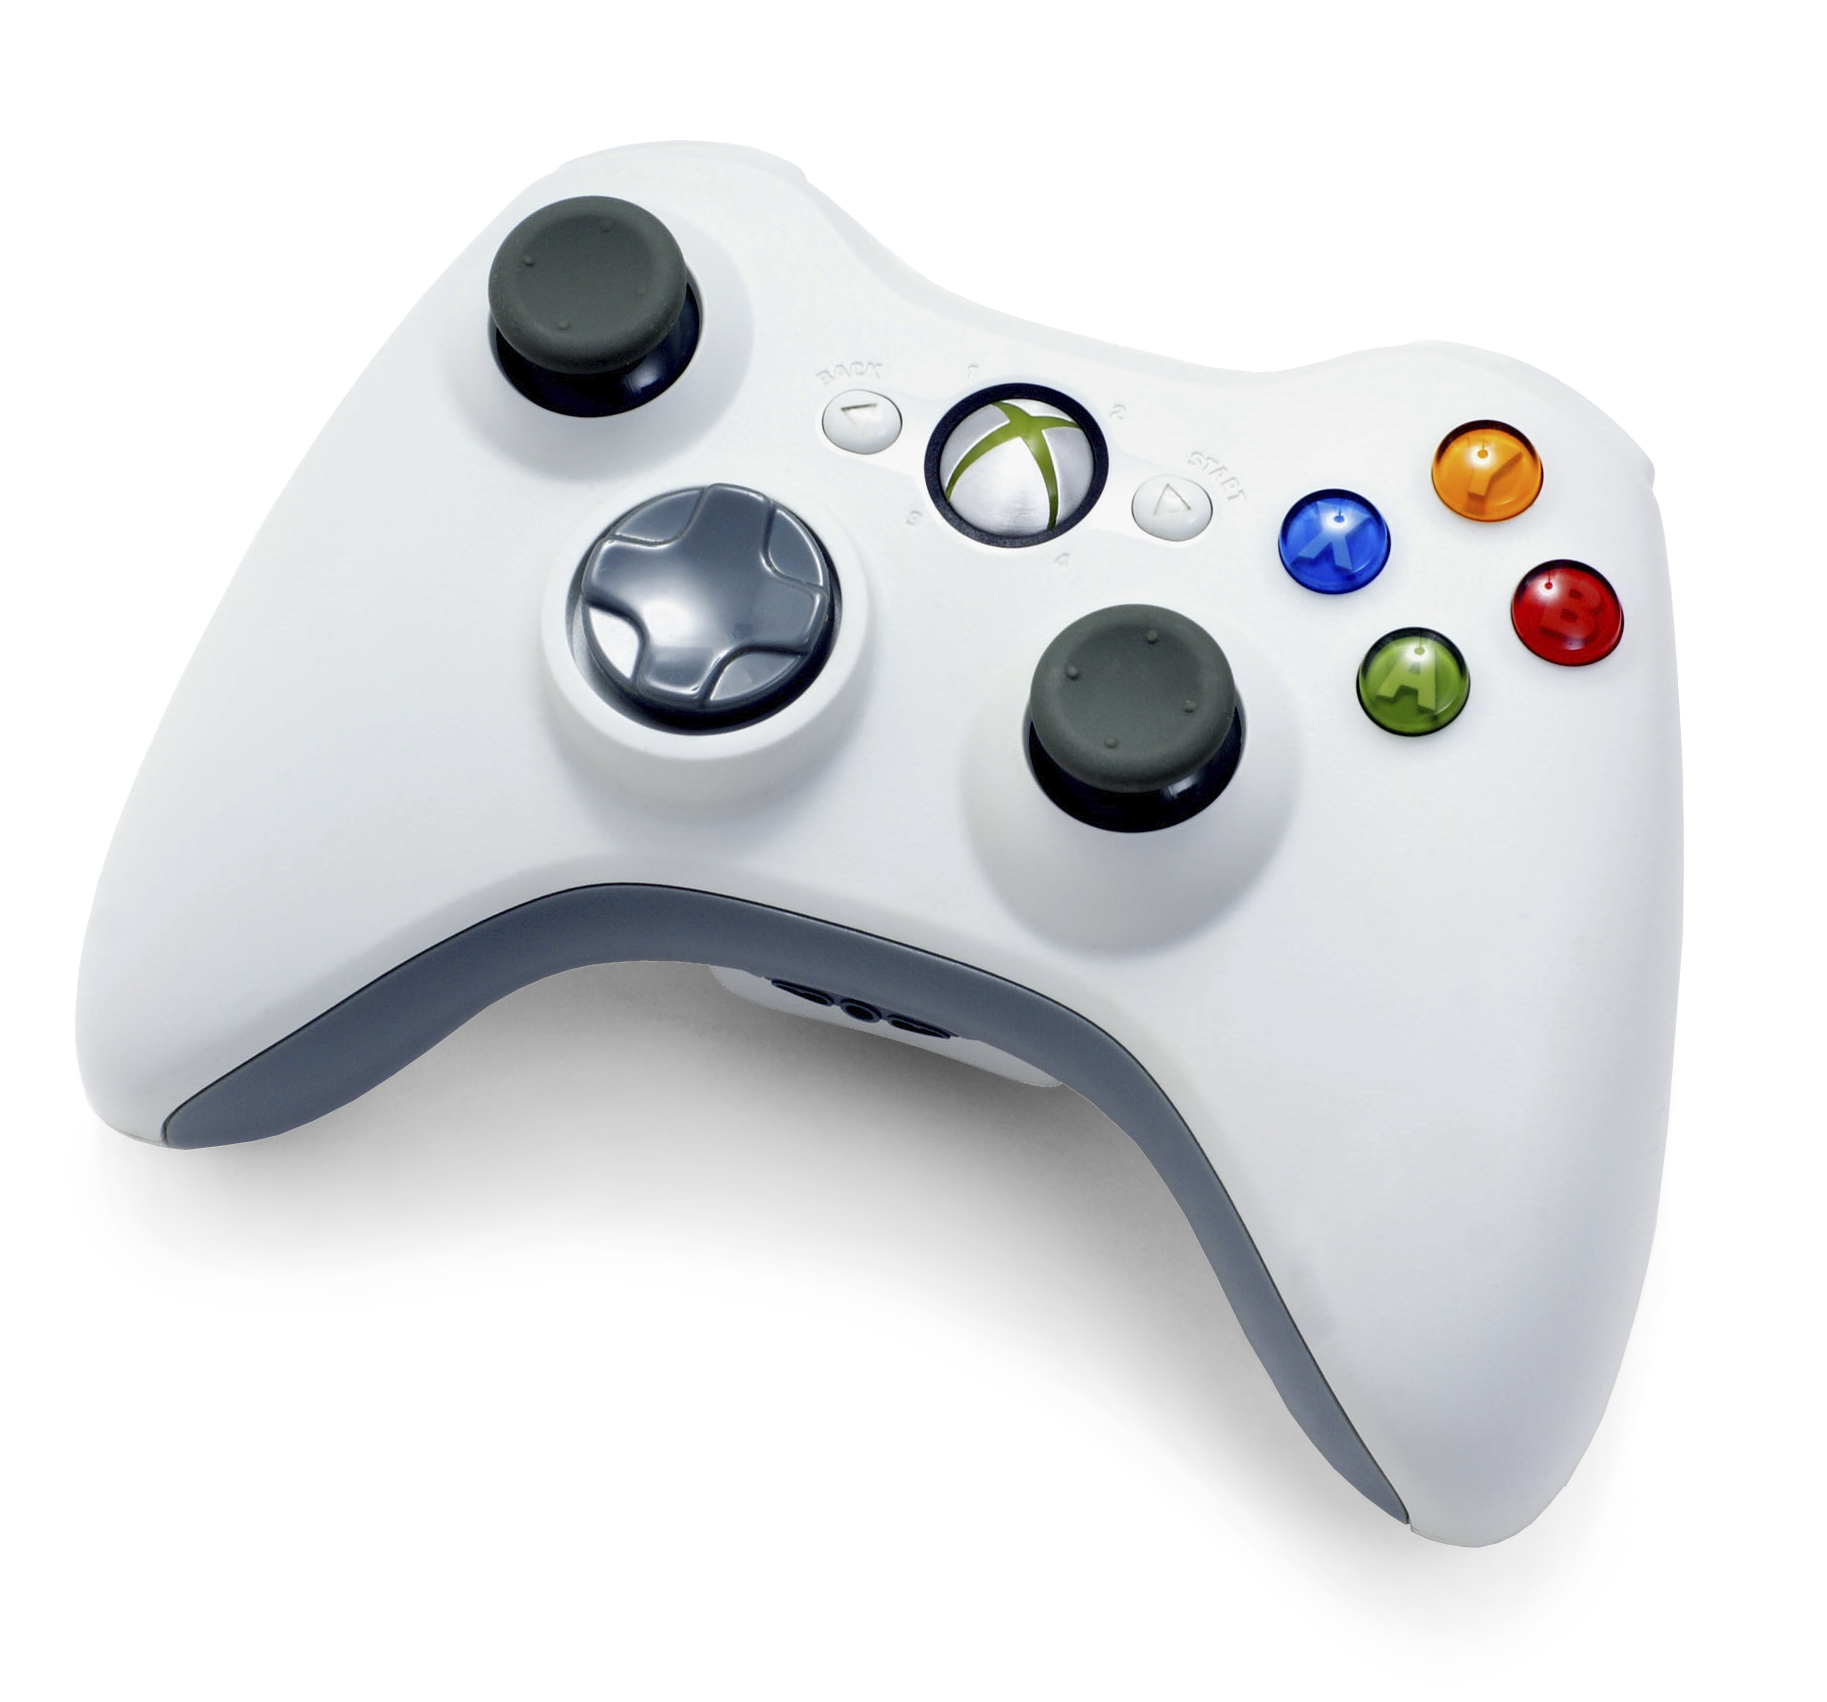
\includegraphics[scale=0.2]{graphics/controller}
  \caption{The Xbox 360 controller, showing the available inputs}
\end{figure}

\subsection{Self-imposed constraints}
We decided to limit ourselves to 2-dimensional graphics, letting us focus more
on architecture and game engine creation than 3-dimensional content creation,
which is a time-consuming process. Additionally, we know from experience that
designing intelligent game AI is relatively time-consuming and challenging.
It is however possible to make captivating games that do not have much in the way
of artificial intelligence in the opponents, so we felt it safe to not prioritize
this. 
